\documentclass[12pt]{article}
\usepackage[italian]{babel}
\usepackage{graphicx}
\usepackage[section]{placeins}
\usepackage{amsmath}% http://ctan.org/pkg/amsmath
\usepackage{enumitem}
\usepackage{graphicx}
\usepackage{hyperref}
\usepackage[section]{placeins}

\title{BISF - Relazione Finale Progetto}
\author{Giuseppe Facchi}
\date{A.A. 2020-2021}

\begin{document}
\maketitle
\newpage
\tableofcontents
\newpage

\section{Data Summary}
La ricerca dei titoli da analizzare è stata effettuata nel mercato borsistico italiano, tra le componenti dell'indice $FTSE.MIB$, iniziato il 31 Dicembre 1992.
Tra tutte le componenti sono state estratte per poi essere esaminate i titoli azionari:
\begin{itemize}
    \item \textbf{TEN.MI}: Tenaris S.A.
    \item \textbf{ENI.MI}: ENI S.p.A.
    \item \textbf{EXO.MI}: Exor N.V.
    \item \textbf{AZM.MI}: Azimut Holding S.p.A.
    \item \textbf{REC.MI}: Recordati Industria Chimica e Farmaceutica S.p.A.
    \item \textbf{DIA.MI}: DiaSorin S.p.A.
\end{itemize}
Il periodo di riferimento per le analisi sarà dal 1 Ottobre 2018 al 1 Ottobre 2020
\subsection{Settore OIL and GAS}
Un settore preso in esame riguarda l'\textbf{OIL and GAS}, influenzato pesantemente dagli effetti della pandemia di SARS-CoV-2. Di questo settore in particolare è stata selezionata \textbf{Tenaris S.A.}, il maggior produttore e fornitore a livello globale di tubi e servizi per l'esplorazione e la produzione di petrolio e gas. Il secondo titolo azionario riguarda invece la multinazionale \textbf{ENI S.p.A.}, attiva nei settori del petrolio, del gas naturale, della chimica e della chimica verde, della produzione e commercializzazione di energia elettrica e delle energie rinnovabili. Nel 2018 è l'ottavo gruppo petrolifero mondiale per giro d'affari.
\begin{figure}[!htb]
    \centering
    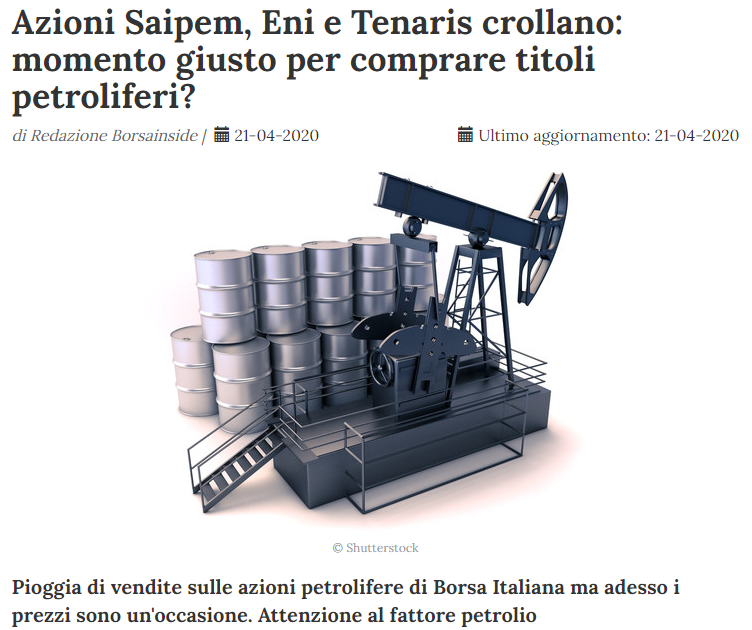
\includegraphics[width=0.8\textwidth]{immagini/eni_ten_news.png}
    \caption{Notizia del 21 Aprile 2020 riguardo il crollo di Tenaris e ENI. \href{https://www.borsainside.com/mercati_italiani/73074-azioni-saipem-eni-tenaris-crollo-momento-giusto-comprare-titoli-petroliferi/}{Link alla notizia}}
\end{figure}
\FloatBarrier

\subsection{Settore FINANCE}
Il secondo settore preso in esame riguarda il settore \textbf{FINANCE}, di cui verranno osservati i titoli azionari di \textbf{Azimut Holding S.p.A.}, una società indipendente che si occupa di consulenza e gestione patrimoniale e \textbf{Exor N.V.}, una holding finanziaria olandese controllata dalla famiglia Agnelli. Oltre al gruppo automotive FCA, i principali investimenti di EXOR includono anche la compagnia di capital good CNH Industrial, il gruppo riassicurativo PartnerRe, la casa automobilistica Ferrari, la squadra di calcio della Juventus, il settimanale The Economist, il gruppo editoriale GEDI, proprietario dei quotidiani la Repubblica, La Stampa, Il Secolo XIX, il settimanale L'Espresso, una catena di quotidiani locali e varie radio. Exor è la prima società in Italia per fatturato, e la 28ª al mondo.
\begin{figure}[!htb]
    \centering
    
\includegraphics[width=0.8\textwidth]{immagini/exor.png}
    \caption{Penali per decine di milioni di dollari per il mancato rispetto del Memorandum of understanding da parte di un'azienda in procinto di essere acquistata da Exor. \href{https://www.ilsole24ore.com/art/exor-salta-l-accordo-covea-la-vendita-partnerre-ADhN48P}{Link alla notizia}}
\end{figure}
\FloatBarrier
\subsection{Settore BIO and TECH}
L'ultimo settore preso in esame riguarda invece il settore \textbf{BIO and TECH}, che contrariamente alla quasi totalità degli altri indici azionari ha registrato una crescita in periodo di pandemia. Di questo settore vengono analizzati i titoli di \textbf{DiaSorin S.p.A.} che opera nei segmenti dell'immunodiagnostica e della diagnostica molecolare ed è a capo di un gruppo composto da 26 società e 4 succursali estere, producendo i propri test in 5 siti produttivi dislocati in Europa e Stati Uniti e di \textbf{Recordati Industria Chimica e Farmaceutica S.p.a.}, una multinazionale farmaceutica italiana fondata nel 1926 con sede a Milano che Sviluppa, produce e commercia prodotti farmaceutici o di chimica farmaceutica.
\begin{figure}[!htb]
    \centering
    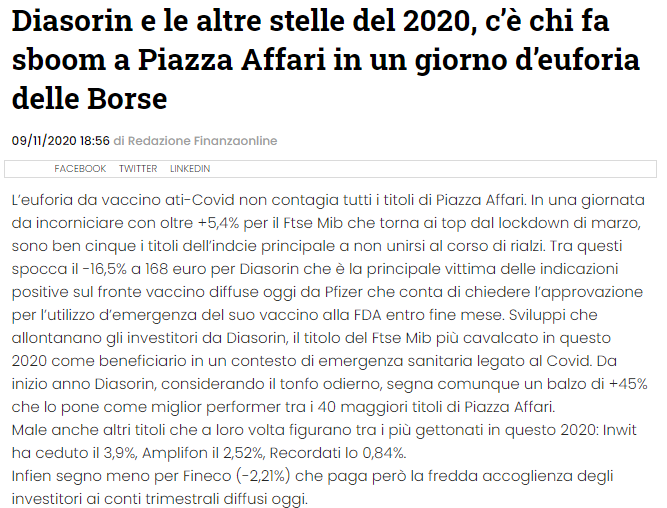
\includegraphics[width=0.8\textwidth]{immagini/dia.png}
    \caption{Rialzi post-covid in borsa dei titoli, ma ribasso pesante di DiaSorin, caso interessante di analisi  \href{https://www.finanzaonline.com/notizie/diasorin-e-le-altre-ecco-chi-fa-sboom-a-piazza-affari-inwit-amplifon-recordati}{Link alla notizia}}
\end{figure}
\FloatBarrier

\begin{figure}[!htb]
    \centering
    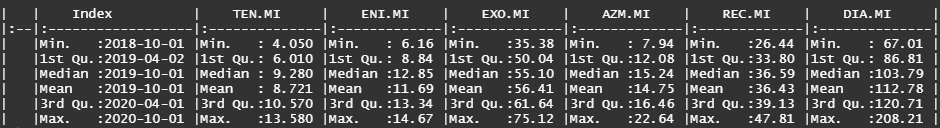
\includegraphics[width=1\textwidth]{immagini/riepilogo.png}
    \caption{Riepilogo degli Adjusted Prices dei titoli azionari in analisi}
\end{figure}
\FloatBarrier
\newpage
\section{Descriptive Analytics}
\FloatBarrier
\begin{figure}[!htb]
    \centering
    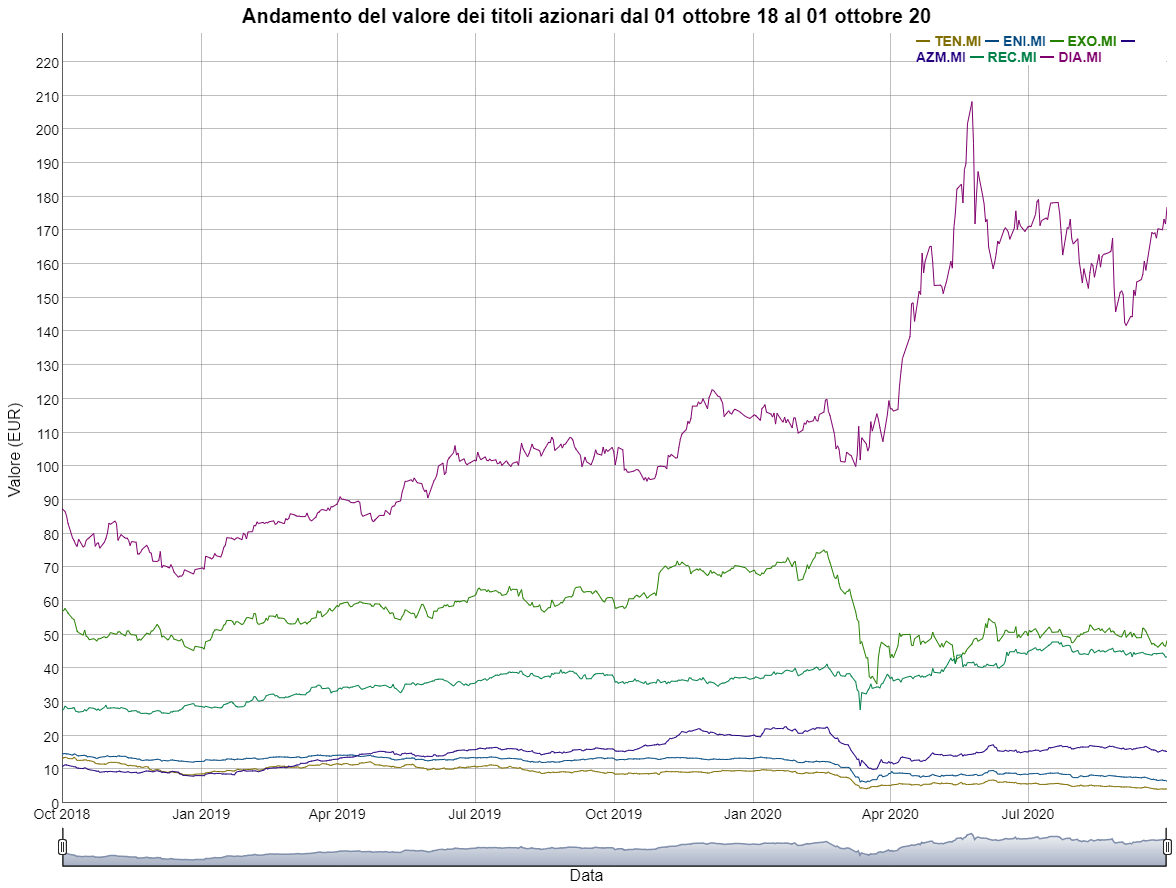
\includegraphics[width=1\textwidth]{immagini/allgraphs.png}
    \caption{Grafico comprendente gli adjusted prices GIORNALIERI dei titoli azionari aggregati dal 1 ottobre 2018 al 1 ottobre 2020}
\end{figure}
\FloatBarrier
Da una prima analisi di questo grafico viene messo in risalto il periodo tra Marzo e Aprile, in corrispondenza dell'inizio della pandemia. Tra tutti i titoli azionari quello di DiaSorin risulta svettare, mentre tutti gli altri subiscono un forte tonfo. Una spiegazione attendibile è data dalla notizia di collaborazione dell'azienda con i principali ospedali italiani per la produzione di uno strumento diagnostico di massa per il COVID.
\href{https://www.repubblica.it/economia/2020/03/10/news/coronavirus_diasorin_annuncia_entro_marzo_test_rapido_in_un_ora-250821897/}{Link alla notizia}
\newpage
\subsection{Analisi dei Ritorni}
Una più precisa analisi può essere effettuata analizzando i grafici dei Compounded Returns. Infatti essi costituiscono una migliore misura delle variazioni di mercato perché indipendenti dalle fluttuazioni assolute di prezzo.
\subsubsection{Granularità Giornaliera}
\begin{figure}[!htb]
    \centering
    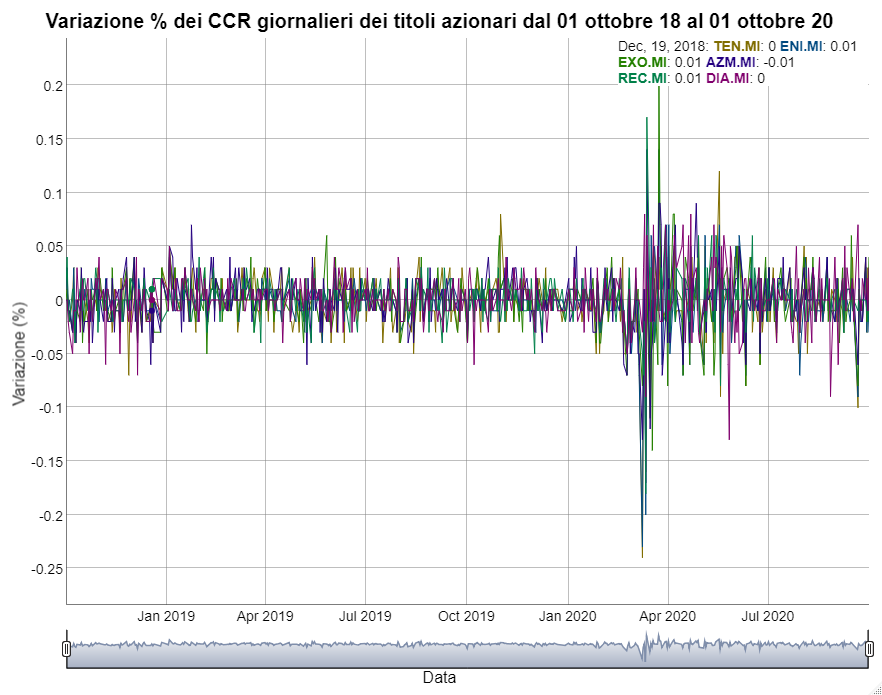
\includegraphics[width=1\textwidth]{immagini/ccrdaily.png}
    \caption{Grafico dei CC Returns Giornalieri dei titoli azionari aggregati dal 1 ottobre 2018 al 1 ottobre 2020}
\end{figure}
\FloatBarrier
\newpage
\subsubsection{Granularità Settimanale}
\begin{figure}[!htb]
    \centering
    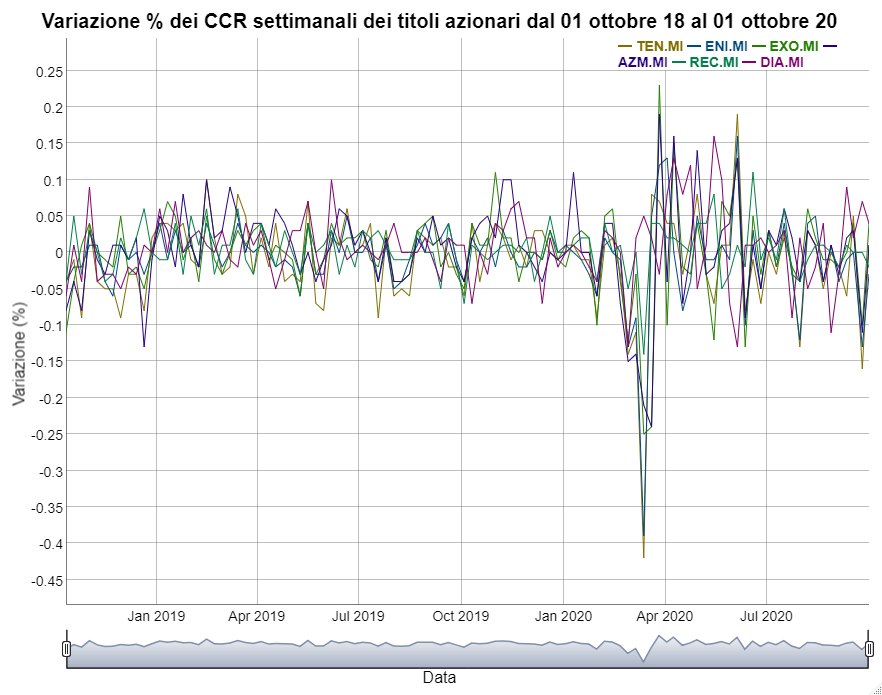
\includegraphics[width=1\textwidth]{immagini/ccrweekly.png}
    \caption{Grafico dei CC Returns Settimanali dei titoli azionari aggregati dal 1 ottobre 2018 al 1 ottobre 2020}
\end{figure}
\FloatBarrier
\newpage
\subsubsection{Granularità Mensile}
\begin{figure}[!htb]
    \centering
    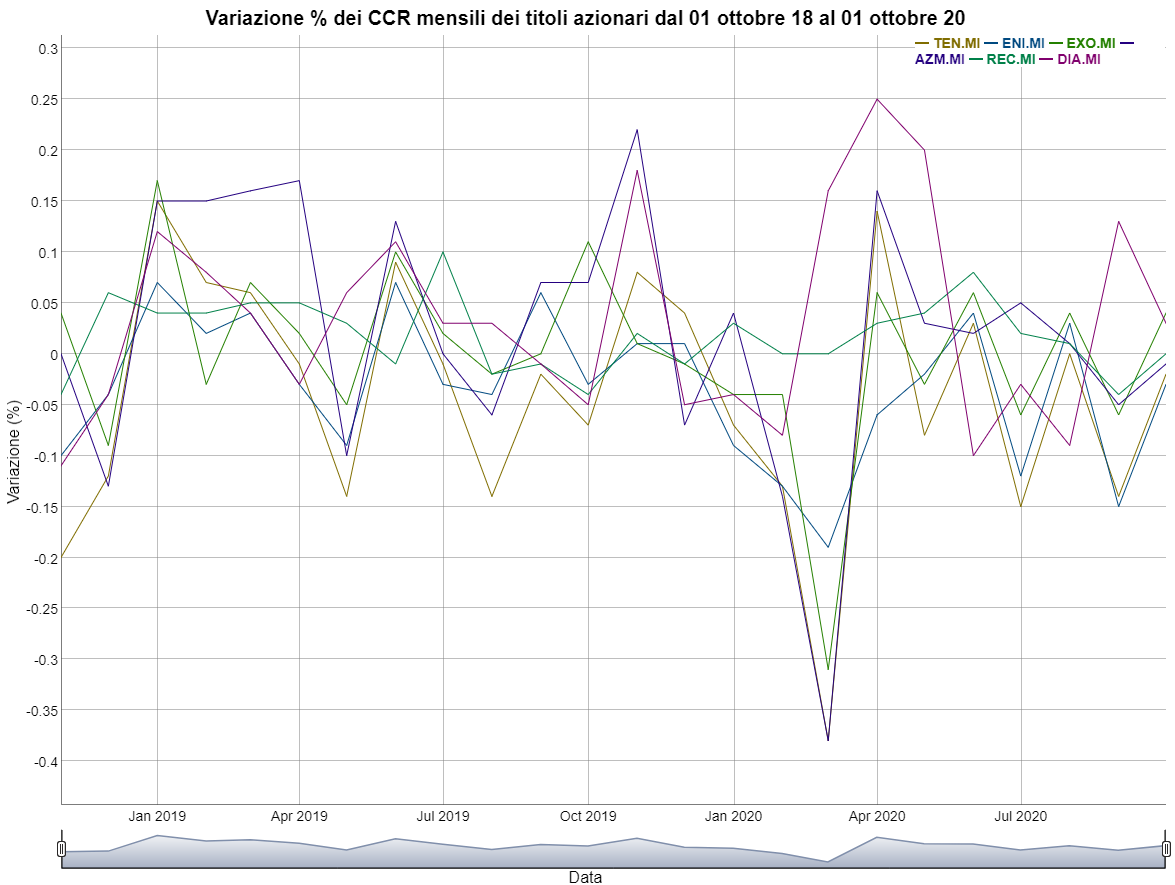
\includegraphics[width=1\textwidth]{immagini/CCRm.png}
    \caption{Grafico dei CC Returns Mensili dei titoli azionari aggregati dal 1 ottobre 2018 al 1 ottobre 2020}
\end{figure}
\FloatBarrier
L'ipotesi formulata nell'analisi del grafico degli Adjusted Close Prices è più precisamente confermata dall'osservazione del grafico dei CCR a granularità mensile.
\newpage
\subsection{Analisi dei settori tramite confronto CCR Mensili}
\subsubsection{Settore OIL and GAS}
\begin{figure}[!htb]
    \centering
    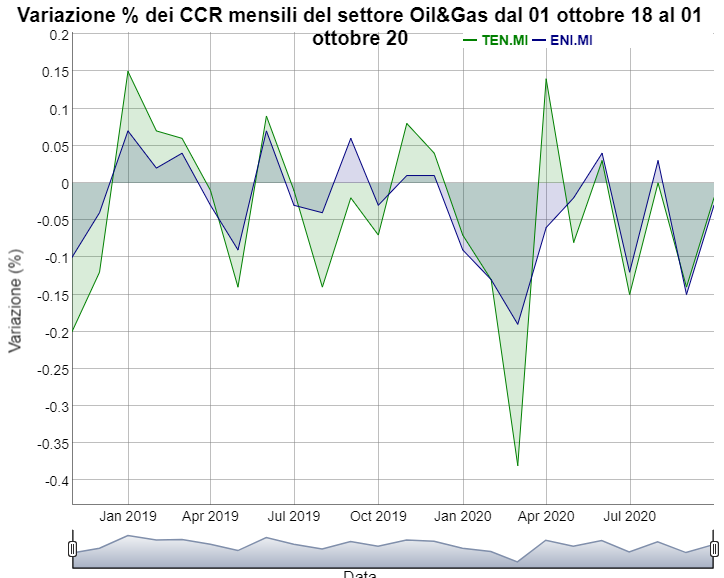
\includegraphics[width=1\textwidth]{immagini/setOil.png}
    \caption{Confronto dei CCR dei titoli del settore Oil and Gas}
\end{figure}
\FloatBarrier
Da questo grafico è possibile notare, a prima vista, una forte correlazione tra i due titoli azionari. Infatti è noto al mercato che l'andamento azionario di Tenaris è molto influenzato dal mercato del petrolio, di cui uno dei maggiori rappresentati è appunto ENI. Tenaris, da questo rapporto di subordinazione, risulta molto più suscettibile alle variazioni di mercato ed è possibile notarlo dalle differenze tra le aree sottese alle linee del grafico.
\newpage
\subsubsection{Settore FINANCE}
\begin{figure}[!htb]
    \centering
    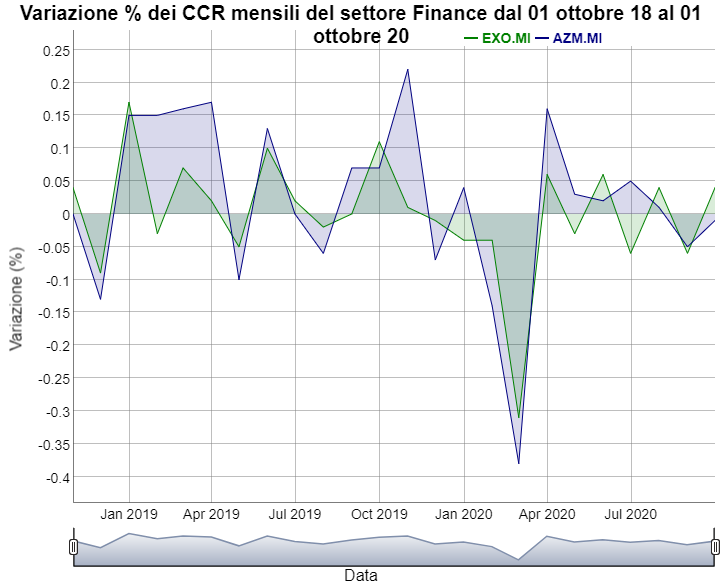
\includegraphics[width=1\textwidth]{immagini/setFin.png}
    \caption{Confronto dei CCR dei titoli del settore Finance}
\end{figure}
\FloatBarrier
In questa situazione si nota, a prima vista, un andamento analogo alla situazione precedente. Le due aziende (Azimut e Exor) non costituiscono però un rapporto di subordinazione, infatti le differenze tra le aree sottese alle linee del grafico sono molto meno estese.
\newpage
\subsubsection{Settore BIO and TECH}
\begin{figure}[!htb]
    \centering
    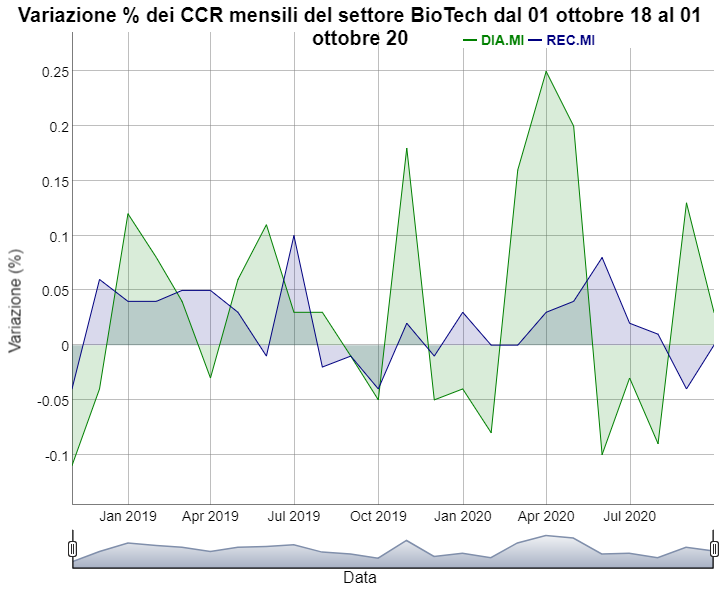
\includegraphics[width=1\textwidth]{immagini/setBio.png}
    \caption{Confronto dei CCR dei titoli del settore Bio and Tech}
\end{figure}
\FloatBarrier
A differenza delle due situazioni precedenti, in questo caso il grafico mostra una certa incorrelazione tra i due titoli anche se facenti parte dello stesso settore produttivo. Questa incorrelazione è data dall'attività produttiva. Infatti per quanto riguarda DiaSorin il picco si ha nel periodo di maggior crisi, quando gli investitori si sono rifugiati nel titolo sperando nell'invenzione di uno strumento diagnostico performante. Per Recordati invece, anche nel periodo di maggiore emergenza, si riscontra un andamento costante, seguendo quello del settore di riferimento. Di una certa importanza è anche la discesa riscontrata da DiaSorin nel periodo intorno Maggio, dovuta allo scandalo che l'ha riguardata. \href{https://www.lastampa.it/cronaca/2020/05/12/news/la-procura-di-milano-indaga-sull-affidamento-dei-test-sierologici-alla-diasorin-1.38835534}{Link alla notizia}
\newpage
\subsection{Analisi di Correlazione}
\subsubsection{Granularità Giornaliera}
\begin{figure}[!htb]
    \centering
    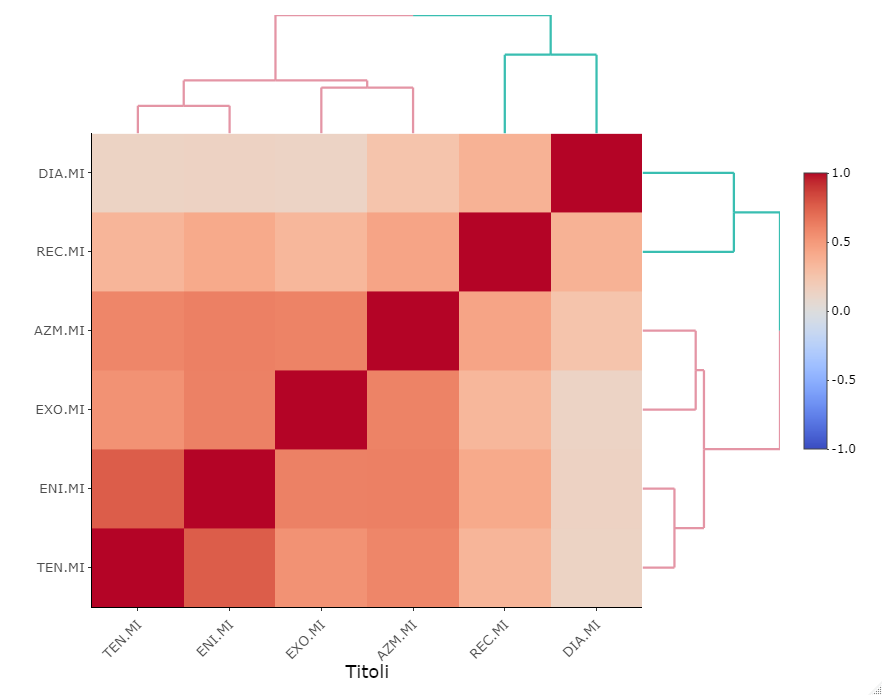
\includegraphics[width=1\textwidth]{immagini/corrdaily.png}
    \caption{Heatmap di correlazione tra i CC Returns a granularità giornaliera dei titoli azionari aggregati dal 1 ottobre 2018 al 1 ottobre 2020}
\end{figure}
\FloatBarrier
Dall'analisi dell'heatmap di correlazione tra i CC Returns a granularità giornaliera dei titoli azionari aggregati dal 1 ottobre 2018 al 1 ottobre 2020 si può dedurre una correlazione abbastanza marcata tra gli stocks dello stesso settore e una correlazione leggermente inferiore tra stocks di diversi settori. In particolare la correlazione tra gli stocks del settore Oil and Gas è quella più marcata, mentre quella tra gli stocks del settore BioTech è quella meno.
\newpage
\subsubsection{Granularità Mensile}
\begin{figure}[!htb]
    \centering
    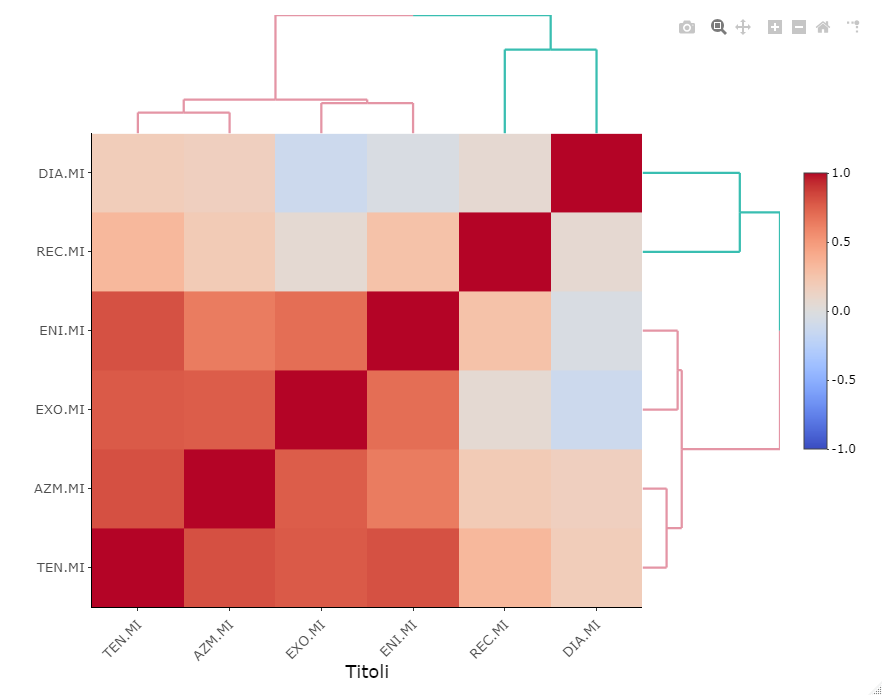
\includegraphics[width=1\textwidth]{immagini/corr_mont.png}
    \caption{Heatmap di correlazione tra i CC Returns a granularità mensile dei titoli azionari aggregati dal 1 ottobre 2018 al 1 ottobre 2020}
\end{figure}
\FloatBarrier
Le osservazioni precedenti vengono riprodotte anche nel caso di analisi di correlazione dei CCR a granularità mensile. La correlazione/incorrelazione riulta addirittura più evidente tra titoli dello stesso settore e, in particolare, si nota una correlazione più marcata tra settore Oil and Gas e settore Finance.
\newpage
\subsection{Statistiche Aggregate}
\begin{figure}[!htb]
    \centering
    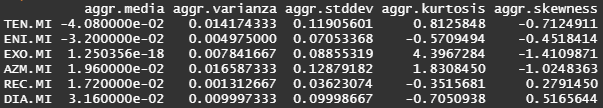
\includegraphics[width=0.9\textwidth]{immagini/stats.png}
    \caption{Statistiche generiche aggregate dei titoli azionari}
\end{figure}
\FloatBarrier
Per una corretta interpretazione dei comportamenti dei titoli azionari è utile considerare le loro generiche statistiche aggregate. Alcune statistiche di degna nota sono:
\begin{itemize}
    \item Titolo con Media di CCR \textit{massima}: \textbf{DIA.MI} con $0.0316\%$
    \item Titolo con Media di CCR \textit{minima}: \textbf{TEN.MI} con $-0.0408\%$
    \item Titolo con Dev. Standard di CCR \textit{massima}: \textbf{AZM.MI} con $0.0196$
    \item Titolo con Dev. Standard di CCR \textit{minima}: \textbf{REC.MI} con $0.0172$
\end{itemize}
\begin{figure}[!htb]
    \centering
    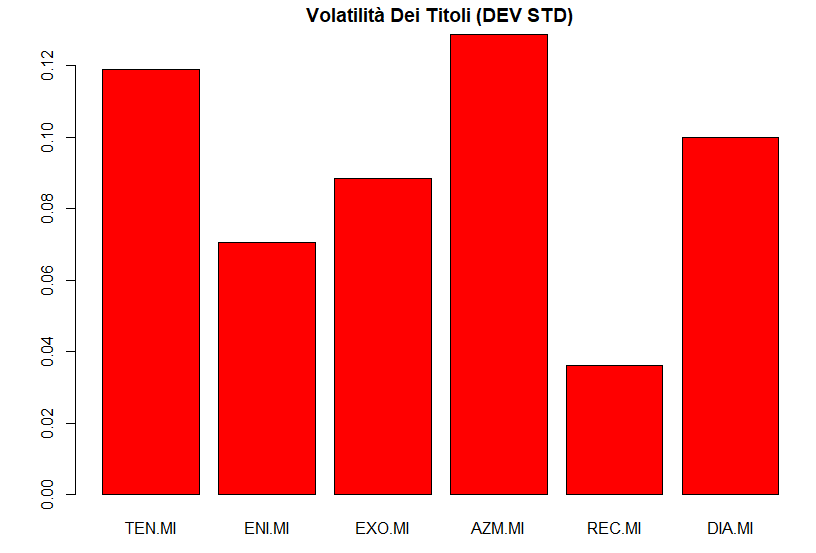
\includegraphics[width=0.8\textwidth]{immagini/volMedia.png}
    \caption{Semplice rappresentazione delle volatilità medie dei titoli}
\end{figure}
\FloatBarrier
\newpage
\subsection{Analisi Aggregata tramite Boxplots}
\begin{figure}[!htb]
    \centering
    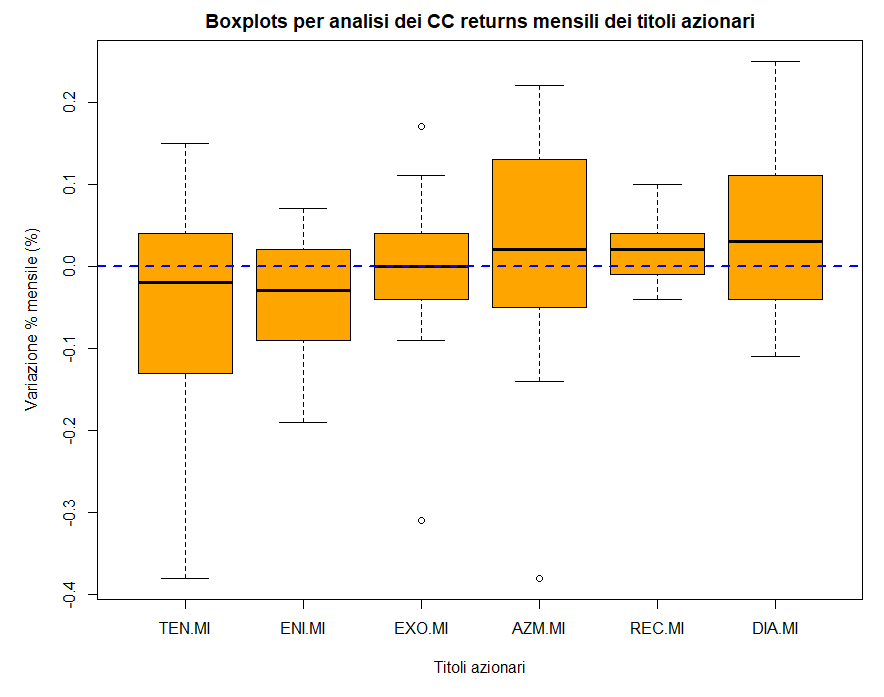
\includegraphics[width=1\textwidth]{immagini/boxplots.png}
    \caption{Boxplots dei titoli azionari}
\end{figure}
\FloatBarrier
Tramite la rappresentazione attraverso boxplots delle distribuzioni dei ritorni dei vari titoli è possibile fare interessanti analisi. Una prima osservazione è possibile farla sui minimi CCR, trovando in Tenaris e Azimut i minimi più marcati e in Recordati il minimo meno marcato. Per Azimut il minimo costituisce un outlier perché non trova una correlazione con la distribuzione degli altri suoi ritorni mensili. Per Tenaris, invece, a parità di minimo, questo non costituisce un elemento eccezionale perché la distribuzione dei ritorni è molto più orientata verso questo valore. Una seconda osservazione è possible effettuarla sulle mediane dei titoli. Le mediane degli stocks sono facilmente considerabili per settori, ritorvando nel settore OIL and GAS mediane negative, nel settore FINANCE una mediana prossima allo 0 e una positiva, e infine nel settore BIOTECH mediane positive. Questa situazione è data dalla maggior presenza, più o meno marcata, di ritorni mensili positivi nelle distribuzioni del settore BIOTECH e FINANCE, e viceversa nel settore OIL and GAS. Per facilitare l'interpretazione delle mediane è stata inserita una retta orizzontale in corrispondenza del ritorno nullo. La seguente osservazione è possibile farla sui massimi CCR, dove la correlazione tra gli stocks è più debole e non è quindi possibile fare considerazioni sui settori, ma solo sui singoli titoli. Un'ultima osservazione riguarda i range di distribuzione, trovando in Tenaris, Azimut e Diasorin i range di distribuzione dei CCR più ampi, mentre nei restanti titoli troviamo range più compressi.
\newpage
\subsection{QQ Plots}
\begin{figure}[!htb]
    \centering
    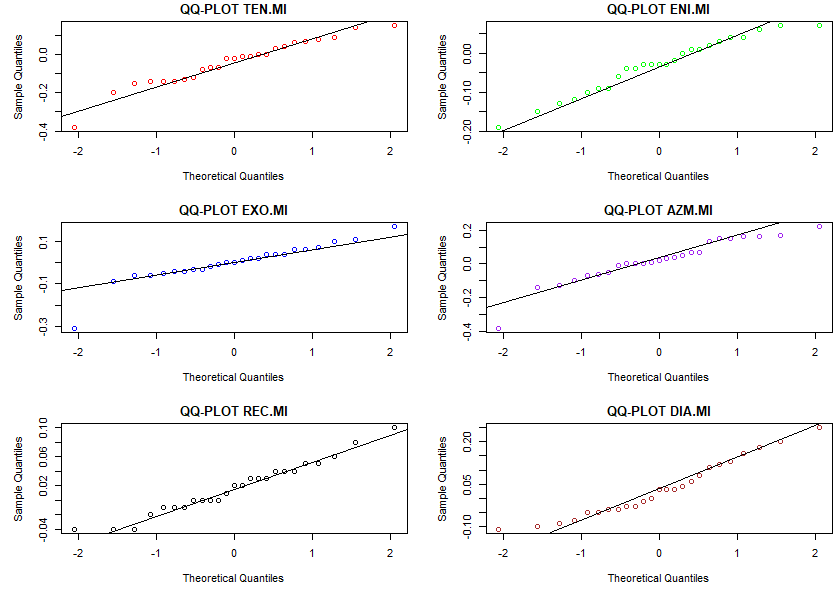
\includegraphics[width=1\textwidth]{immagini/qq.png}
    \caption{QQ Plots dei titoli azionari}
\end{figure}
\FloatBarrier
Utile ai fini dell'analisi degli stocks è la comparazione delle distibuzioni dei CCR mensili rispetto alla distibuzione normale. Anche se in presenza di alcuni valori che si discostano dalla retta (outliers) è possibile approssimare le varie distribuzioni dei CCR a una normale. Sarà quindi necessario proseguire con analisi dettagliate tramite l'utilizzo di altri strumenti.
\newpage
\subsection{Analisi diagnostiche sui singoli titoli}
Per analizzare meglio l'andamento dei titoli, è utile considerare le distribuzioni dei CCR. A questo scopo possono aiutare istogrammi di frequenza, boxplots e QQ plots.
\subsubsection{TEN.MI}
\begin{figure}[!htb]
    \centering
    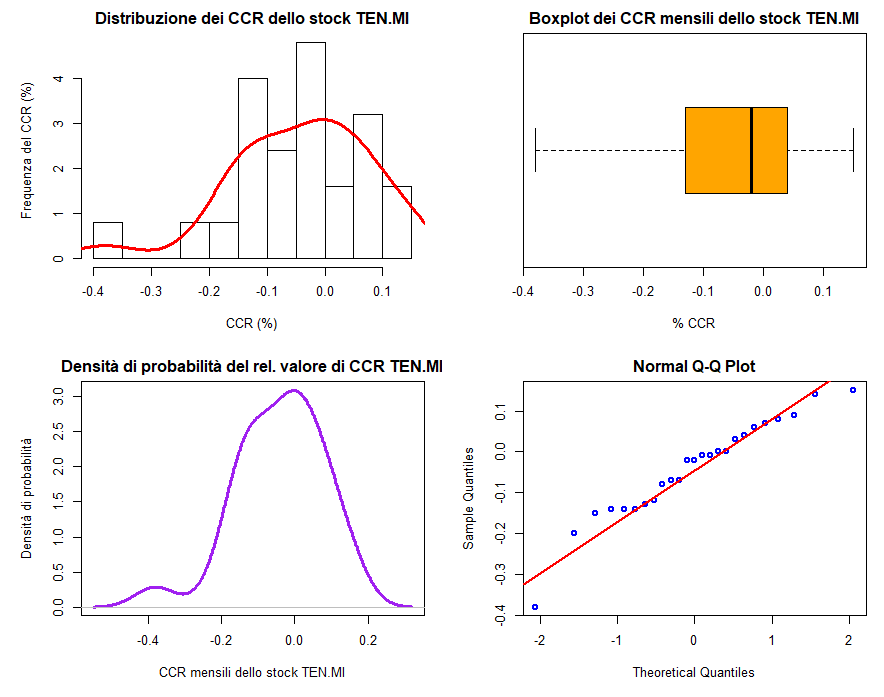
\includegraphics[width=1\textwidth]{immagini/diag_ten.png}
    \caption{Diag TEN}
\end{figure}
\FloatBarrier
Per quanto riguarda Tenaris, si può osservare una distribuzione dei ritorni molto simile ad una distribuzione normale, con l'assenza di outliers e una mediana dei CCR poco al di sotto dello 0. In particolare si può osservare una presenza maggiore di ritorni minori della mediana (già negativa) nel primo quartile di distribuzione e un minimo che si discosta dalla delimitazione del primo quartile molto di più di quello che fa il massimo.
\newpage
\subsubsection{ENI.MI}
\begin{figure}[!htb]
    \centering
    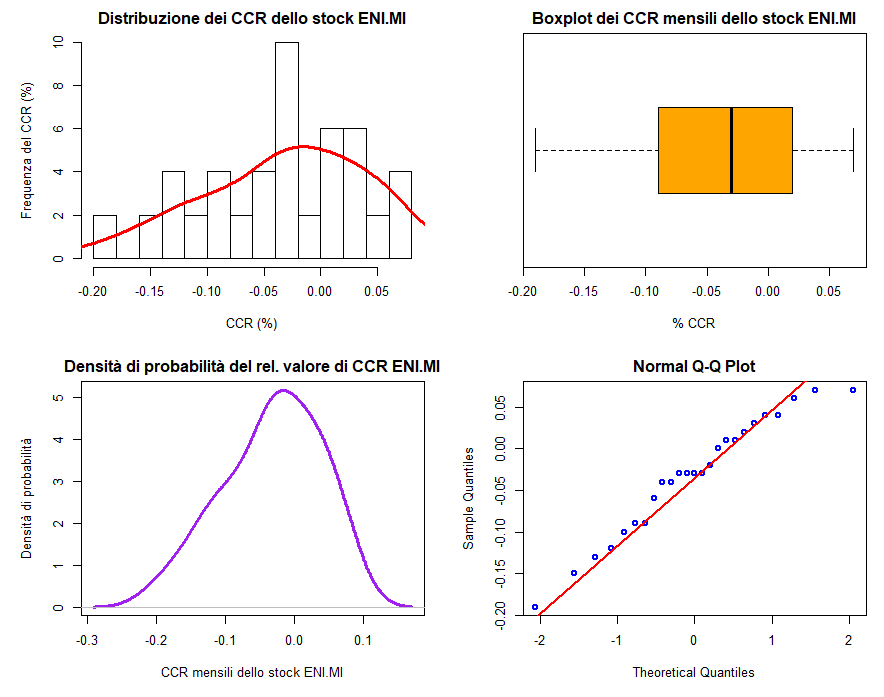
\includegraphics[width=1\textwidth]{immagini/diag_eni.png}
    \caption{Diag ENI}
\end{figure}
\FloatBarrier
Per quanto riguarda ENI, invece, troviamo una distribuzione di CCR molto più limitata rispetto a Tenaris. Questo può essere confermato osservando che il range dei CCR varia da circa $-0.2$ a $0.1$ anche se con una media pressoché simile, quindi negativa. Possibile anche osservare che i CCR sono distributi secondo una normale.
\newpage
\subsubsection{EXO.MI}
\begin{figure}[!htb]
    \centering
    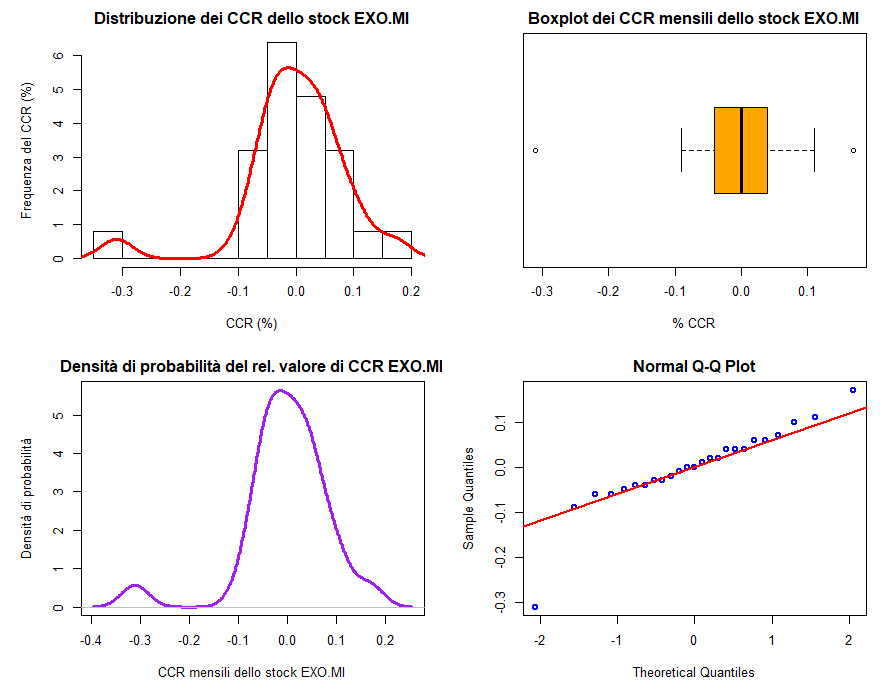
\includegraphics[width=1\textwidth]{immagini/diag_exo.png}
    \caption{Diag EXO}
\end{figure}
\FloatBarrier
Nel settore Finance è possibile trovare conferma di quello osservato precedentemente nei boxplots aggregati. Infatti il range di distribuzione dei CCR risulta molto più ristretto anche se vi è la presenza di outliers. Nel caso di Exor l'outlier in corrispondenza del ritorno di $-3\%$ è dovuto al periodo di crisi dei mercati dovuto al COVID, mentre l'outlier positivo, in corrispondenza dello $0.2\%$ circa, è in linea con l'andamento del settore finanziario nel primo mese 2019. La mediana dei ritorni si attesta vicina allo 0 con un massimo ritorno che si discosta più del minimo ritorno.
\newpage
\subsubsection{AZM.MI}
\begin{figure}[!htb]
    \centering
    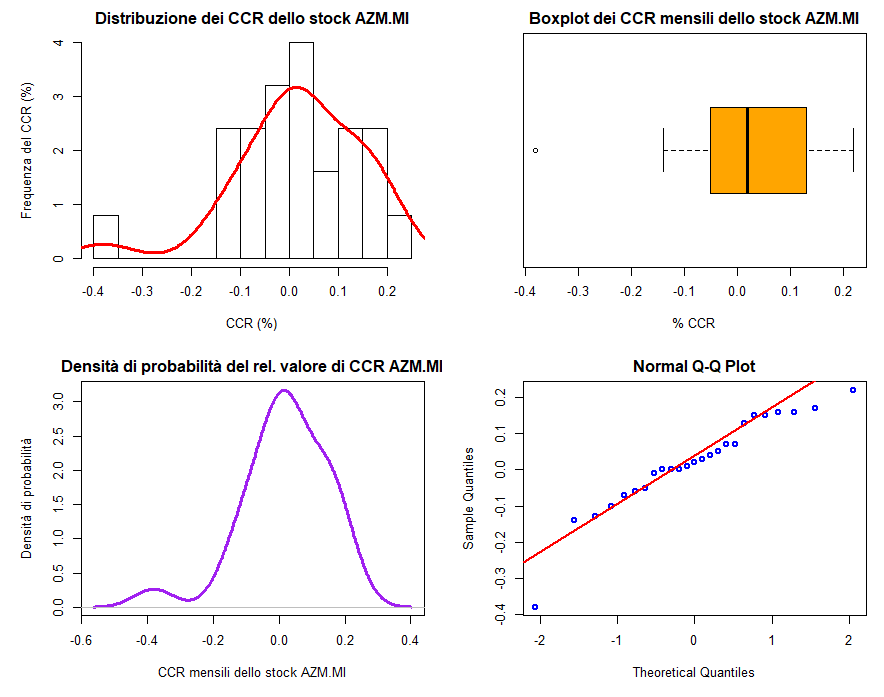
\includegraphics[width=1\textwidth]{immagini/diag_azm.png}
    \caption{Diag AZM}
\end{figure}
Per quanto riguarda il titolo di Azimut Holdings valgono le considerazioni fatte per Exor, anche se possiamo osservare che non è presente l'outlier positivo che invece ritroviamo per Exor. L'outlier negativo che si ritrova per il titolo è anche qui dovuto al periodo COVID, generando un ritorno negativo eccezionale per lo stock. Questo outlier è possibile anche riscontrarlo nell'analisi del QQ-plot come lo spot più basso del grafico.
\FloatBarrier
\newpage
\subsubsection{REC.MI}
\begin{figure}[!htb]
    \centering
    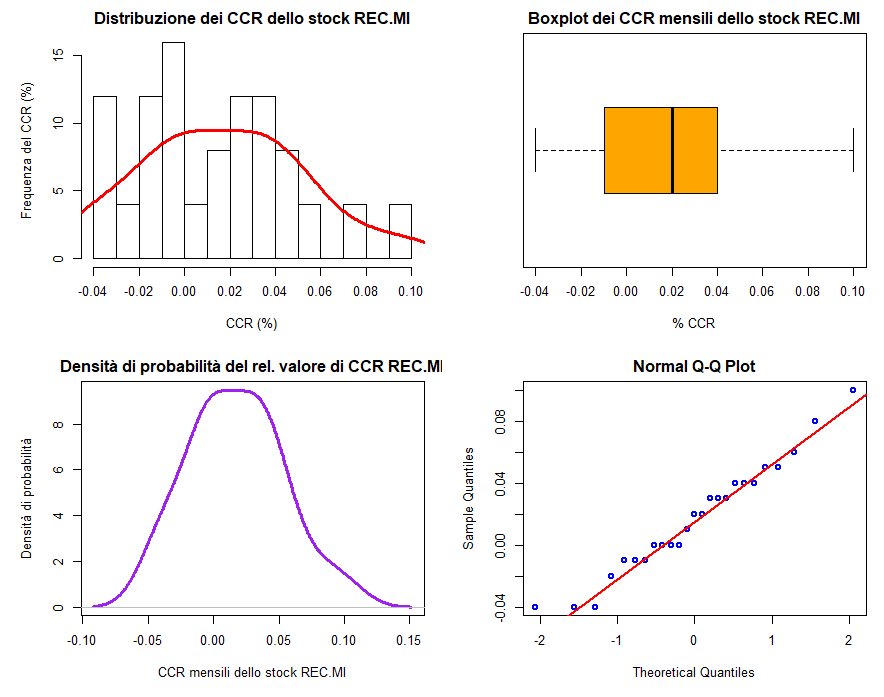
\includegraphics[width=1\textwidth]{immagini/diag_rec.png}
    \caption{Diag REC}
\end{figure}
\FloatBarrier
Passando al settore Biotech il range di distibuzione dei ritorni si amplia maggiormente, con mediane positive e massimi che si discostano dai boxplots più di quanto si discostino i minimi. Recordati presenta una distribuzione di CCR con una mediana intorno al $2\%$ e un massimo del $10\%$ nel periodo di luglio 2019. In particolare Venerdì 12 luglio la società farmaceutica ha annunciato la firma di un accordo con Novartis per l’acquisizione a livello mondiale dei diritti per i farmaci Signifor e Signifor LAR. L’accordo prevede anche l’acquisizione dei diritti a livello mondiale di osilodrostat. \href{https://www.soldionline.it/notizie/azioni-italia/performance-recordati-15-luglio-2019}{Link alla notizia}. Anche qui viene osservata una distribuzione dei CCR approssimabile ad una normale.
\newpage
\subsubsection{DIA.MI}
\begin{figure}[!htb]
    \centering
    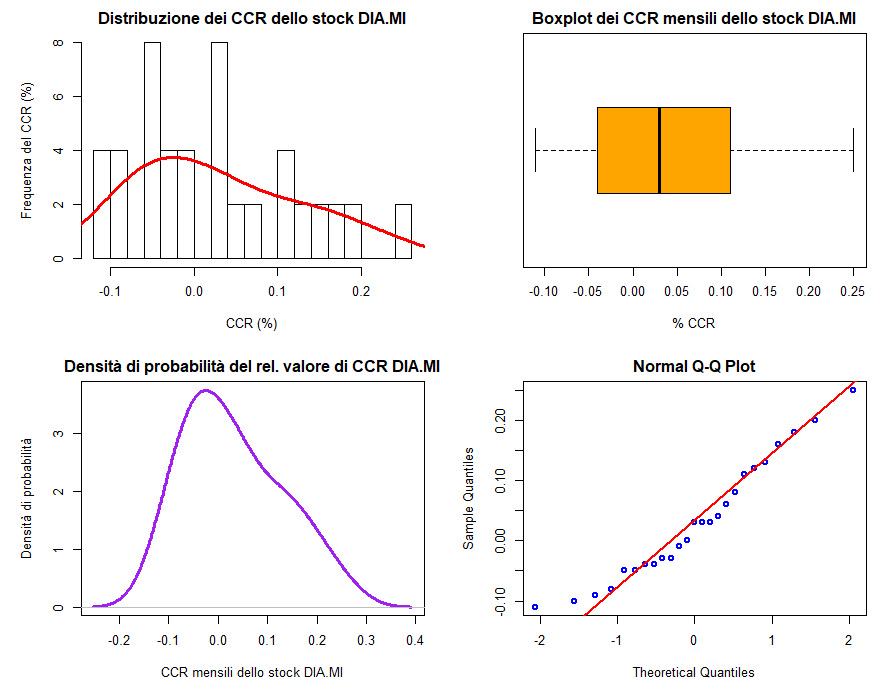
\includegraphics[width=1\textwidth]{immagini/diag_dia.png}
    \caption{Diag DIA}
\end{figure}
\FloatBarrier
Il titolo di DiaSorin presenta le stesse caratteristiche del titolo di Recordati, tranne che per una differenza sostanziale riguardo il ritorno massimo che, in questo caso, risulta molto più rilevante per la notizia riportata nell'introduzione. La mediana è postiva e si attesta intorno al $5\%$, presentando un ritorno massimo che si discosta più di quanto si discosti il ritorno minimo.
\newpage
\section{Predictive Analytics}
\subsection{Predizione tramite ARIMA}
Mediante l'utilizzo di un modello autoregressivo integrato a media mobile (ARIMA) è possibile fare una previsione sull'andamento dei CCR degli stocks sulla base dei CCR già in possesso. Per raggiungere questo obiettivo è necessario ampliare il dataset in analisi includendo i valori dei CCR antecedenti alla data iniziale di riferimento (dal 2007). Il processo di forecasting in questione prende in analisi, per quanto riguarda questa soluzione, 80 mesi di training set (da ottobre 2010 a maggio 2017), 30 di test (giugno 2017 a dicembre 2019) e 10 (da gennaio 2020 a ottobre 2020, data di termine analisi) di vero e proprio forecasting. Sulla base dei CCR di training l'approccio utilizzato del forecasting prevede l'utlizzo dei modelli ARMA, dopo il confronto con i CCR di test, con minor RMSE per ogni stock e il vero e proprio forecasting usando i modelli precedentemente computati sui CCR concatenati di training e test. La prima fase consiste nel calcolare i modelli ARMA con RMSE minimo per ogni stock. Per questa analisi sono stati considerati i parametri come segue:
\begin{itemize}
    \item $0\leq AR \leq 10$
    \item $I=0$
    \item $0\leq MA \leq 10$
\end{itemize}
Da cui sono stati ricavate le seguenti migliori configurazioni:
\begin{figure}[!htb]
    \centering
    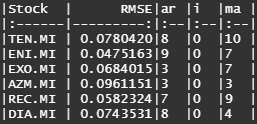
\includegraphics[width=0.5\textwidth]{immagini/rmse.png}
    \caption{Migliori configurazioni ARIMA per gli stock in analisi}
\end{figure}
\FloatBarrier
\subsubsection{TEN.MI}
La previsione ARIMA, per quanto riguarda TEN.MI, ha dato il seguente risultato per $n$ mesi (30)
\begin{figure}[!htb]
    \centering
    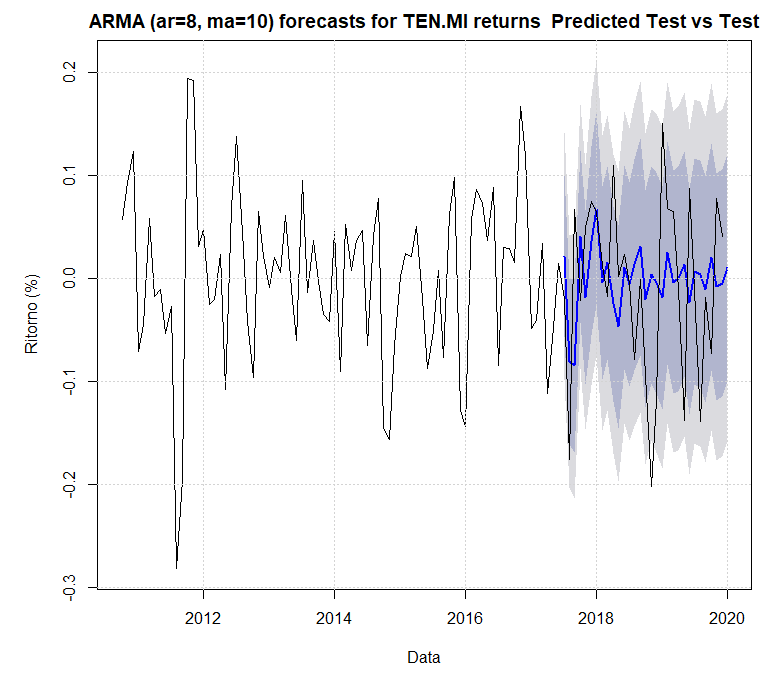
\includegraphics[width=1\textwidth]{immagini/tenmiforecast.png}
    \caption{Plot del forecast di $m$ mesi per TEN.MI che ha dato RMSE minore tra CCR predetti e di test}
\end{figure}
\FloatBarrier
Utilizzando questo modello è stato poi eseguito il forecast vero e proprio sugli $l$ mesi successivi (10), producendo questo risultato:
\begin{figure}[!htb]
    \centering
    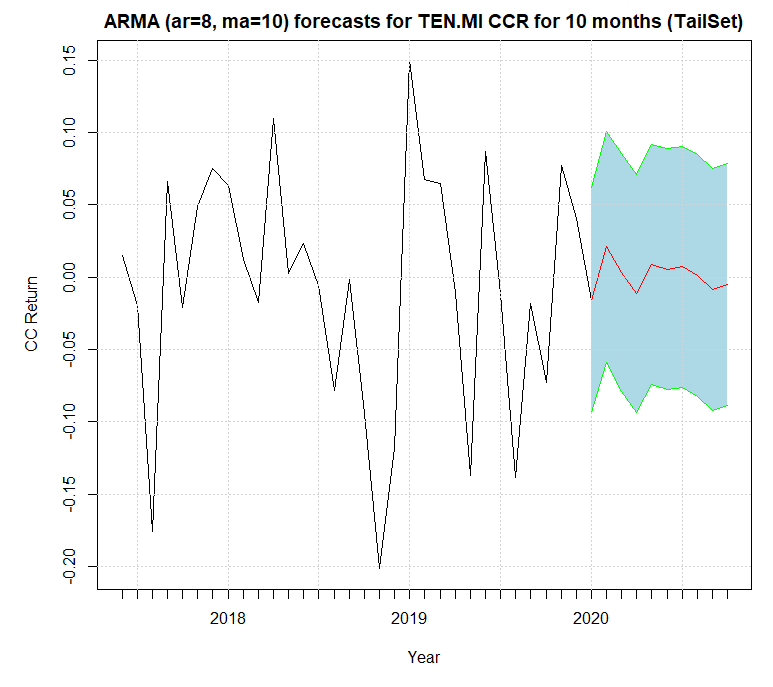
\includegraphics[width=1\textwidth]{immagini/tenmiL.png}
    \caption{Plot del forecast di $l$ mesi per TEN.MI utilizzando il modello ARIMA con migliore RMSE tra dati di test e predetti}
\end{figure}
Un'ulteriore analisi sull'efficacia del forecast è quindi condotta confrontando i valori di CCR reali degli $l$ mesi con quelli predetti da ARIMA
\begin{figure}[!htb]
    \centering
    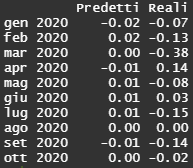
\includegraphics[width=0.3\textwidth]{immagini/predvsreal.png}
    \caption{Confronto tra i valori di CCR prodotti da ARIMA per gli $l$ mesi e i CCR reali}
\end{figure}
\FloatBarrier
Calcolando anche i ritorni cumulati sui 10 mesi è possibile fare un confronto dei ritorni aggregati.
\begin{figure}[!htb]
    \centering
    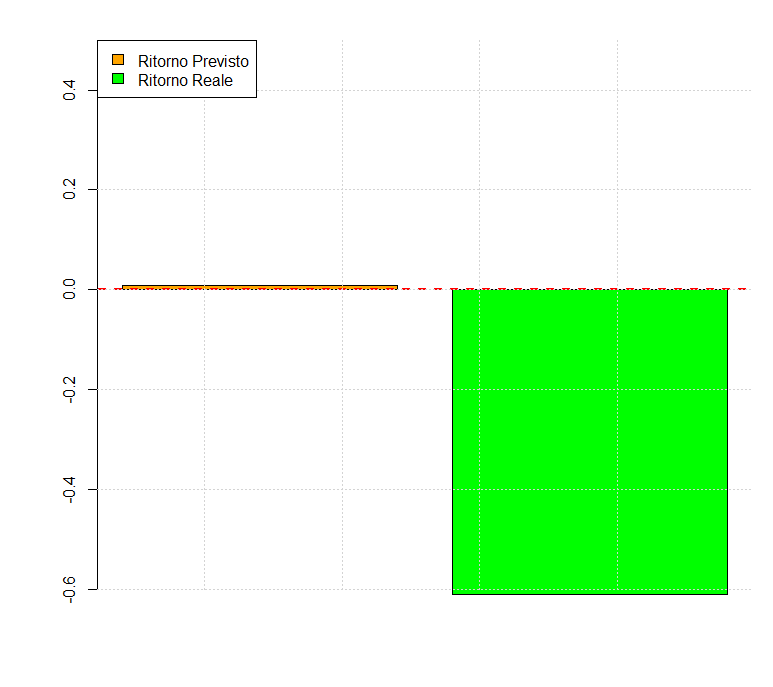
\includegraphics[width=0.8\textwidth]{immagini/tenmiplotrp.png}
    \caption{Confronto tra i ritorni cumulati predetti da ARIMA per gli $l$ mesi e i CCR cumulati reali}
\end{figure}
\FloatBarrier
Com'è possibile notare dal grafico, si è formata una cospicua discrepanza tra valori reali e valori predetti. Questa situazione è sicuramente causata dagli avvenimenti del 2020, che hanno influito molto sulla stagionalità dei ritorni e quindi hanno contribuito a creare un modello di predizione non efficace. Questo è possibile notarlo anche per la maggior parte degli altri stocks.
\newpage
\subsubsection{ENI.MI}
\begin{figure}[!htb]
    \centering
    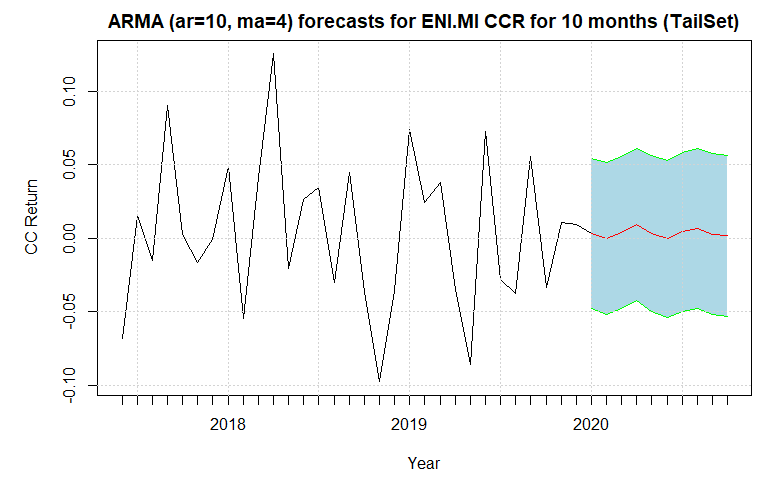
\includegraphics[width=0.8\textwidth]{immagini/foreENI.png}
    \caption{Confronto tra i valori di CCR prodotti da ARIMA per gli $l$ mesi e i CCR reali}
\end{figure}
\FloatBarrier
\begin{figure}[!htb]
    \centering
    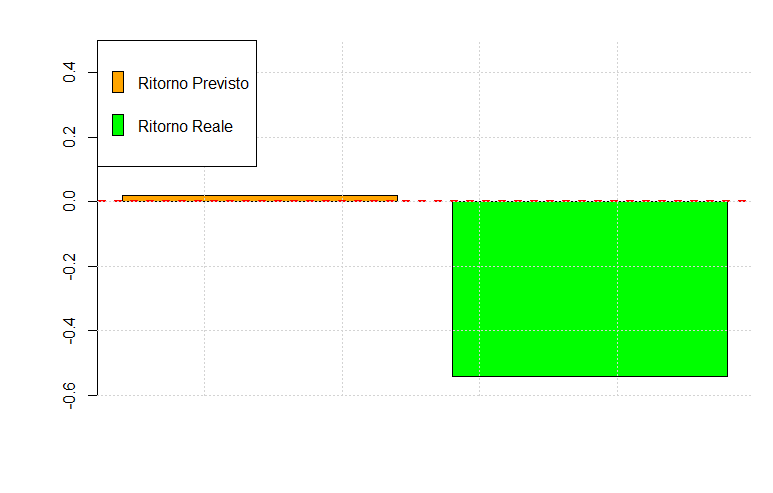
\includegraphics[width=0.8\textwidth]{immagini/foreENIbar.png}
    \caption{Confronto tra i ritorni cumulati predetti da ARIMA per gli $l$ mesi e i CCR cumulati reali}
\end{figure}
\FloatBarrier
Le stesse considerazioni fatte per TEN.MI possono essere riprese per ENI.MI
\subsubsection{EXO.MI}
\begin{figure}[!htb]
    \centering
    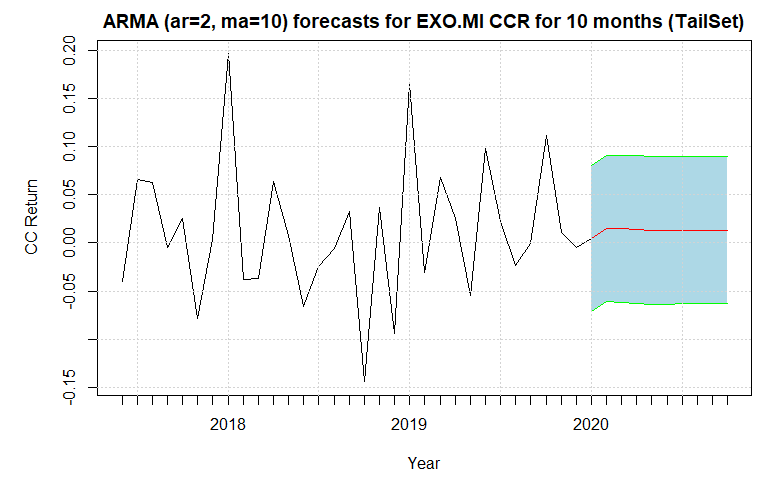
\includegraphics[width=0.8\textwidth]{immagini/foreEXO.png}
    \caption{Confronto tra i valori di CCR prodotti da ARIMA per gli $l$ mesi e i CCR reali}
\end{figure}
\FloatBarrier
Per quanto riguarda EXO.MI il modello ARIMA con RMSE minimo offre un forecast molto approssimativo, questo è dovuto soprattutto alla presenza di outliers nei CCR mensili del titolo.
\begin{figure}[!htb]
    \centering
    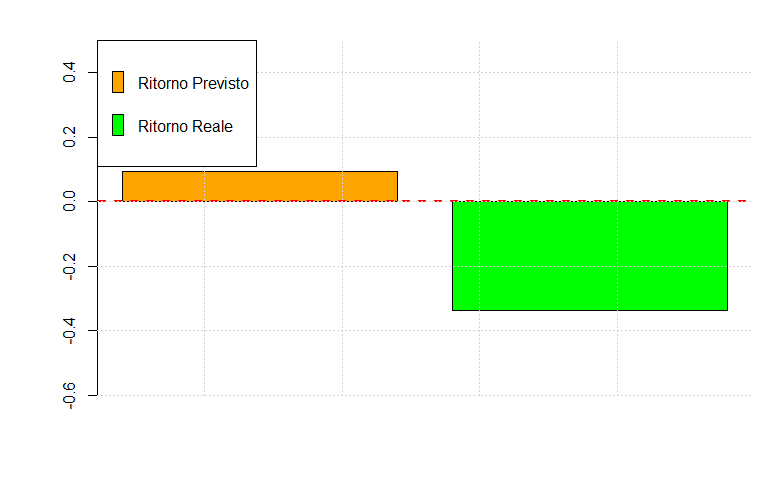
\includegraphics[width=0.8\textwidth]{immagini/foreEXObar.png}
    \caption{Confronto tra i ritorni cumulati predetti da ARIMA per gli $l$ mesi e i CCR cumulati reali}
\end{figure}
\FloatBarrier
\subsubsection{AZM.MI}
\begin{figure}[!htb]
    \centering
    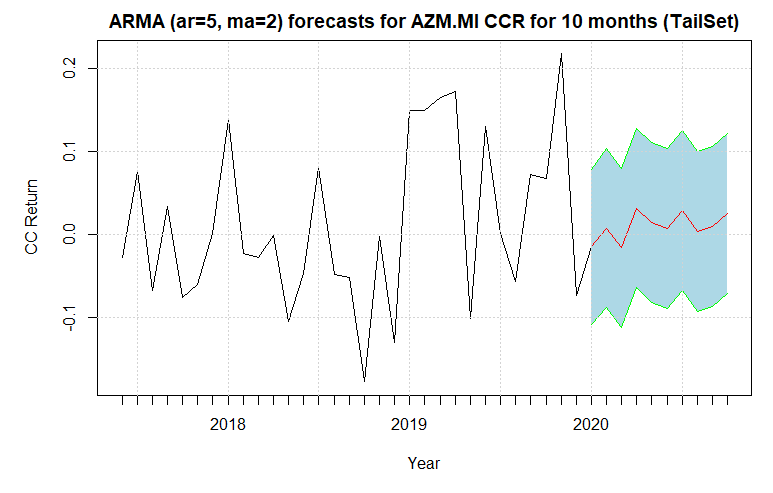
\includegraphics[width=0.8\textwidth]{immagini/foreAZM.png}
    \caption{Confronto tra i valori di CCR prodotti da ARIMA per gli $l$ mesi e i CCR reali}
\end{figure}
\FloatBarrier
\begin{figure}[!htb]
    \centering
    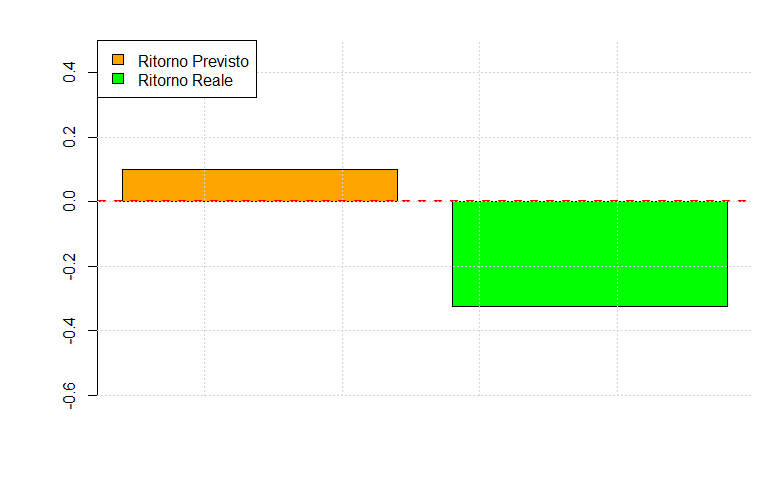
\includegraphics[width=0.8\textwidth]{immagini/foreAZMbar.png}
    \caption{Confronto tra i ritorni cumulati predetti da ARIMA per gli $l$ mesi e i CCR cumulati reali}
\end{figure}
\FloatBarrier
\subsubsection{REC.MI}
\begin{figure}[!htb]
    \centering
    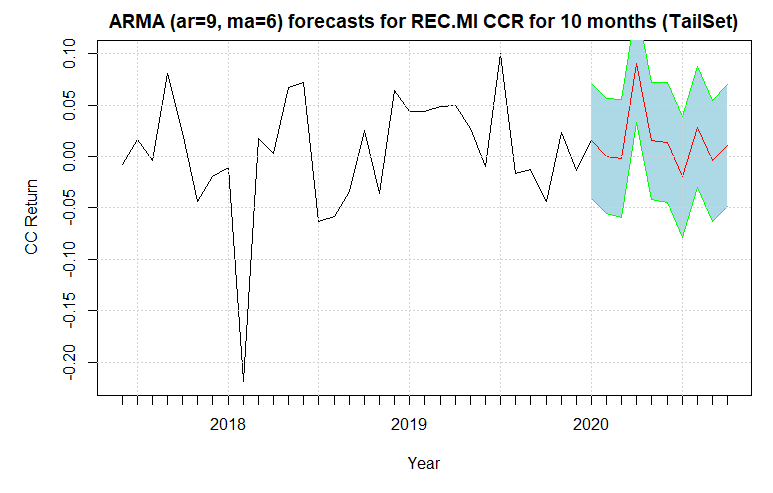
\includegraphics[width=0.8\textwidth]{immagini/foreREC.png}
    \caption{Confronto tra i valori di CCR prodotti da ARIMA per gli $l$ mesi e i CCR reali}
\end{figure}
\FloatBarrier
\begin{figure}[!htb]
    \centering
    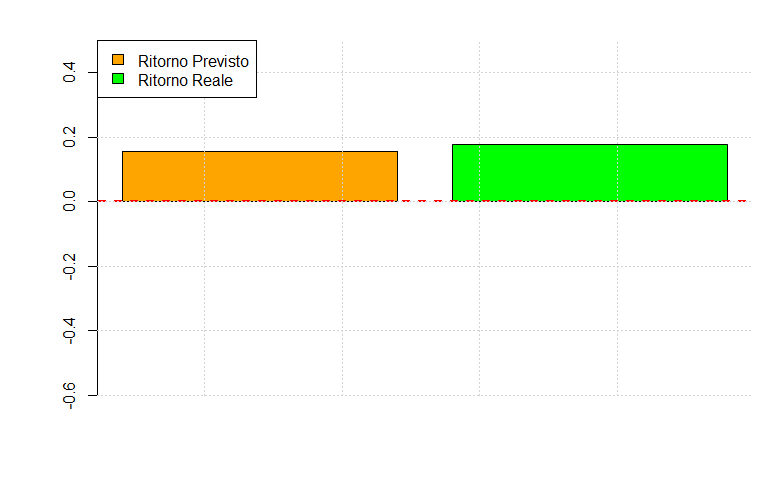
\includegraphics[width=0.8\textwidth]{immagini/foreRECbar.png}
    \caption{Confronto tra i ritorni cumulati predetti da ARIMA per gli $l$ mesi e i CCR cumulati reali}
\end{figure}
\FloatBarrier
Per il settore farmaceutico è possibile notare come i ritorni previsti non si discostino molto dai ritorni reali. Questo perché il settore non ha risentito della crisi COVID nel 2020.
\newpage
\subsubsection{DIA.MI}
\begin{figure}[!htb]
    \centering
    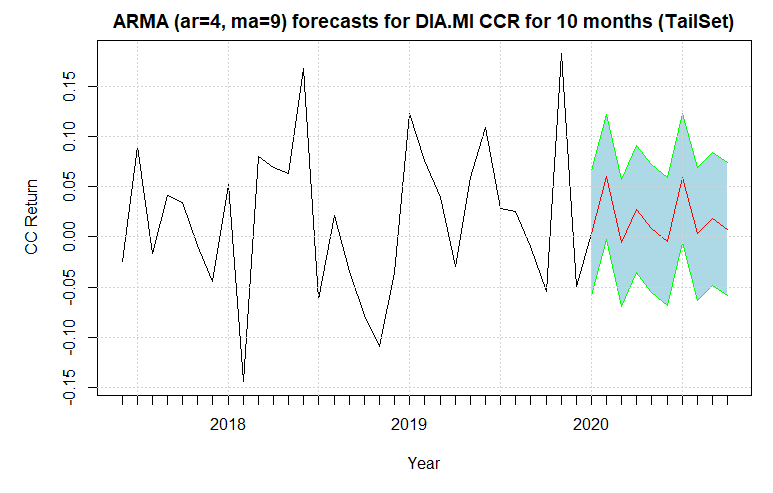
\includegraphics[width=0.8\textwidth]{immagini/foreDIA.png}
    \caption{Confronto tra i valori di CCR prodotti da ARIMA per gli $l$ mesi e i CCR reali}
\end{figure}
\FloatBarrier
\begin{figure}[!htb]
    \centering
    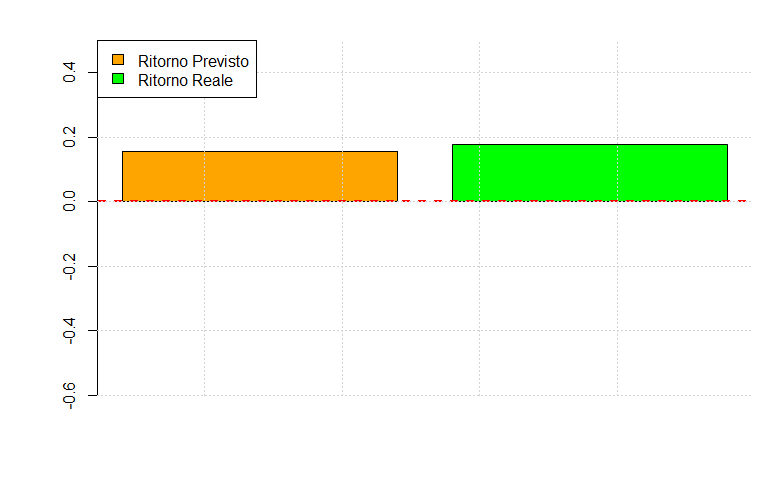
\includegraphics[width=0.8\textwidth]{immagini/foreDIAbar.png}
    \caption{Confronto tra i ritorni cumulati predetti da ARIMA per gli $l$ mesi e i CCR cumulati reali}
\end{figure}
\FloatBarrier
\subsection{Beta}
Utile ai fini di analisi è la computazione del parametro Beta. Per il relativo calcolo è necessario conoscere i CCR dell'indice di mercato di riferimento (FTSE.MIB) per la finsetra temporale considerata per gli stocks. È possibile quindi calcolare Beta per l'intera finestra temporale, ottenendo i seguenti risultati:
\begin{figure}[!htb]
    \centering
    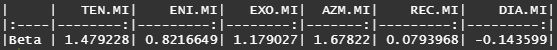
\includegraphics[width=0.9\textwidth]{immagini/beta20182020.png}
    \caption{Valori di Beta per l'arco temporale in analisi}
\end{figure}
\FloatBarrier
Facendo riferimento alla figura 25, è possibile analizzare gli stocks secondo il parametro Beta
\begin{figure}[!htb]
    \centering
    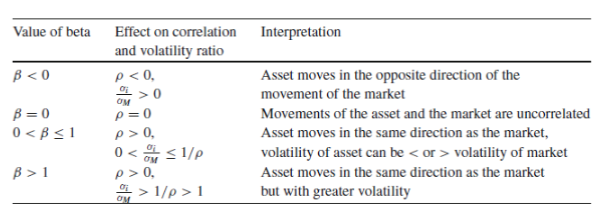
\includegraphics[width=1\textwidth]{immagini/beta.png}
    \caption{Significati di $\beta$}
\end{figure}
\FloatBarrier
\begin{itemize}
    \item TEN.MI, con un $\beta > 1$ si muove nella stessa direzione del mercato, ma con un'alta volatilità
    \item ENI.MI, con un $\beta$ compreso tra 0 e 1 si muove nella stessa direzione del mercato ma non si può concludere nulla sulla sua volatilità
    \item EXO.MI, con un $\beta > 1$ si muove nella stessa direzione del mercato, ma con un'alta volatilità
    \item AZM.MI, con un $\beta > 1$ si muove nella stessa direzione del mercato, ma con un'alta volatilità
    \item Il movimento di REC.MI, con un $\beta \approx 0$, è incorrelato rispetto al movimento del mercato
    \item DIA.MI, con un $\beta < 0$ si muove in direzione opposta rispetto al mercato
\end{itemize}
È possibile anche analizzare Beta secondo intervalli più brevi, come nell'esempio seguente, dove la finestra temporale è di 6 mesi. Per ogni finestra temporale l'analisi di Beta rispecchia l'andamento correlato del mercato per quell'intervallo. Infatti il valore di Beta di un determinato mese viene calcolato utilizzando i ritorni della finestra temporale di ampiezza 6 mesi precedenti.
\begin{figure}[!htb]
    \centering
    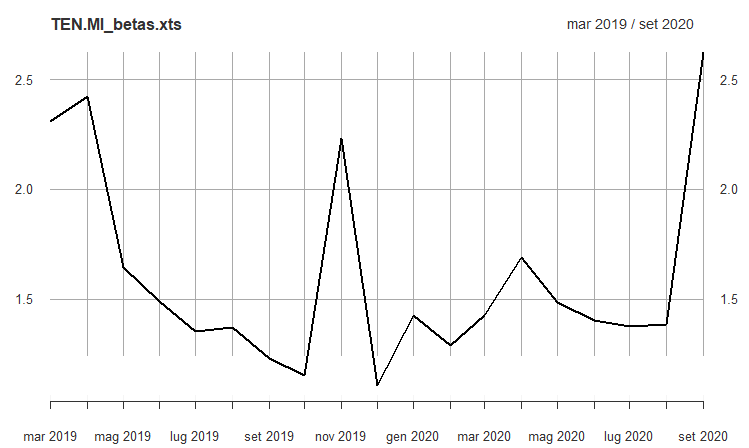
\includegraphics[width=1\textwidth]{immagini/betaTenMIfinestratotale.png}
    \caption{Computazione di $\beta$ per finestre temporali di 6 mesi di TEN.MI}
\end{figure}
\FloatBarrier


\newpage
\section{Portfolio Management}
\subsection{Portfolio Optimization}
La data di costituzione del portfolio fa riferimento all'inizio degli $l$ mesi presi in considerazione per il forecasting. La strategia di portfolio optimization segue il modello di Markowitz e prevede quindi una suddivisione dei pesi dei titoli secondo questo schema, calcolato utilizzando gli adjusted close prices degli stocks dall'inizio disponibilità:
\begin{figure}[!htb]
    \centering
    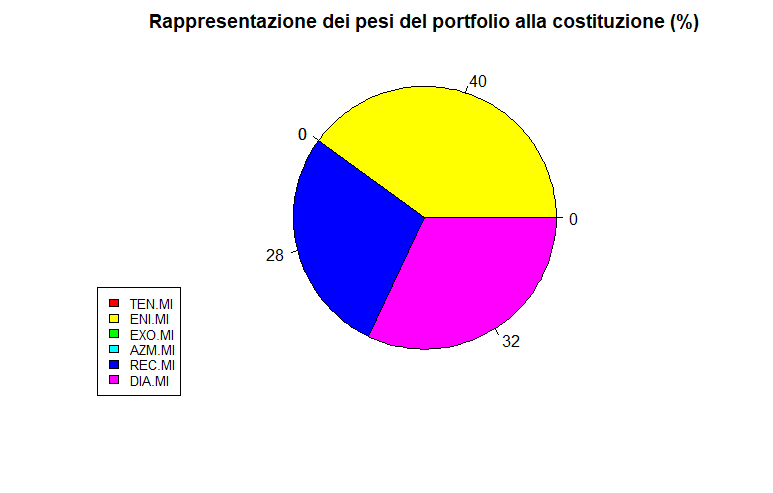
\includegraphics[width=1\textwidth]{immagini/weights.png}
    \caption{Ripartizione dei pesi del portfolio secondo Markowitz alla data di costituzione}
\end{figure}
\FloatBarrier
Di seguito anche la costituzione della frontiera di efficienza, e il posizionamento del Market Portfolio. Dall'analisi del MP si evince che il suo ritorno atteso si aggira intorno al $15\%$.
\begin{figure}[!htb]
    \centering
    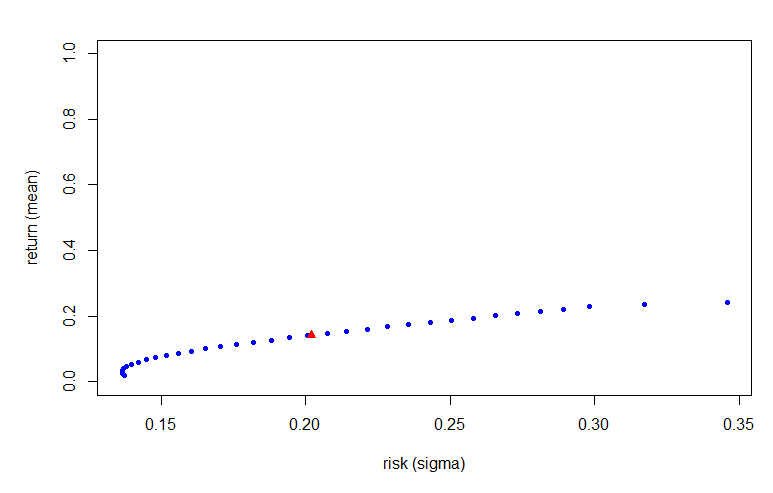
\includegraphics[width=1\textwidth]{immagini/frontiera.png}
    \caption{Frontiera efficiente con MP secondo Markowitz}
\end{figure}
\FloatBarrier

\subsection{Strategia di investimento}
Come strategia di investimento, in questa analisi, è prevista una buy-and-hold dalla costituzione del portfolio fino alla fine della finestra temporale in analisi. Come budget è stata considerata una quota di 5000€ e dei costi di transazione al $3\%$.
In base al precedente calcolo dei pesi ottimali per l'investimento è possibile computare il numero di shares per stock e la relativa spesa. Qui di seguito viene riportato il loro calcolo (con applicati i relativi costi di transazione):
\begin{itemize}
    \item \textbf{TEN.MI}: 0 quote a 9.044246 € cad. $\Rightarrow 0$ €
    \item \textbf{ENI.MI}: 149 quote a 12.96299 € cad. $\Rightarrow 1989.43$ €
    \item \textbf{EXO.MI}: 0 quote a 69.11371 € cad. $\Rightarrow 0$ €
    \item \textbf{AZM.MI}: 0 quote a 21.06253 € cad. $\Rightarrow 0$ €
    \item \textbf{REC.MI}: 37 quote a 35.96073 € cad. $\Rightarrow 1370.46$ €
    \item \textbf{DIA.MI}: 12 quote a 121.4059 € cad. $\Rightarrow 1500.57$ €
\end{itemize}
Da questi dati è possibile estrapolare sia spesa che residuo (quota non utilizzata per l'investimento) relativi all'investimento
\begin{figure}[!htb]
    \centering
    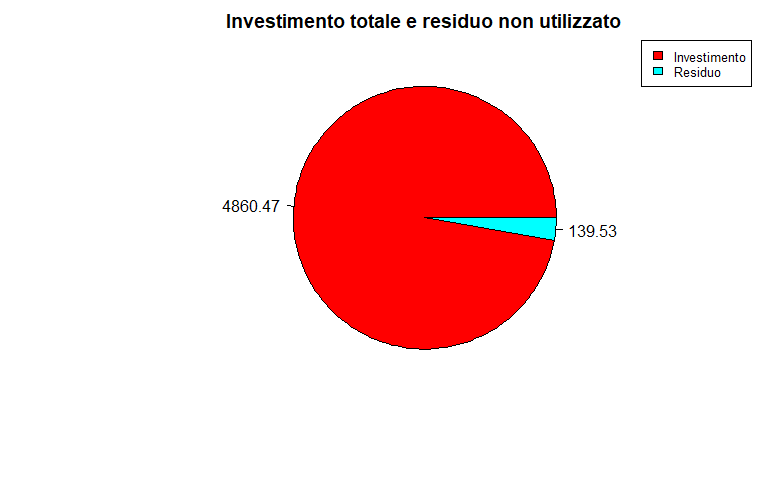
\includegraphics[width=1\textwidth]{immagini/invres.png}
    \caption{Investimento totale e residuo non utilizzato (€)}
\end{figure}
\FloatBarrier
Il valore del portfolio alla fine del periodo risulta però essere minore a quello iniziale ed è pari a $4690.81$ €, con una differenza di $169,66$ €. Questo succede perché all'atto di costituzione del portfolio (l'inizio degli $l$ mesi) la combinazione ottimale per il portfolio è data dai dati fino a quel momento storico, non sapendo degli effetti causati dalla pandemia. Il relativo ritorno reale corrisponde allo $-2.65\%$. Utile ai fini di analisi è il confronto tra ritorno atteso cumulato del Portfolio Optimized, il ritorno previsto mediante ARIMA cumulato usando come pesi quelli dati dalla portfolio optimization e i ritorni reali veri e propri, per poterne poi estrarre delle considerazioni.
\begin{figure}[!htb]
    \centering
    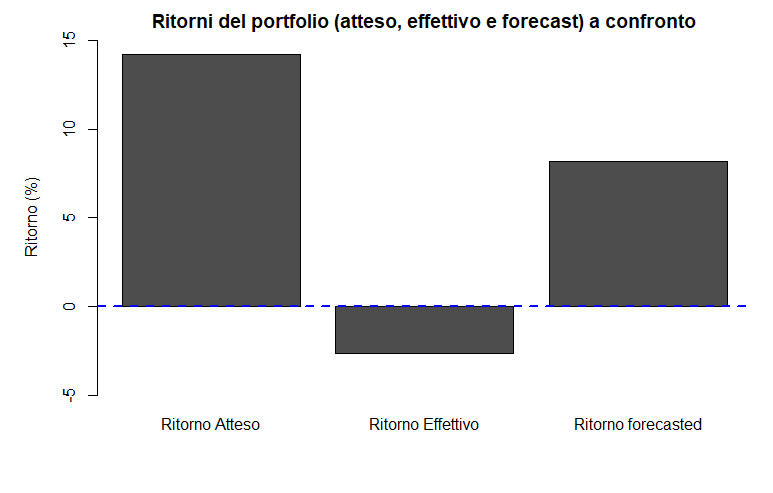
\includegraphics[width=1\textwidth]{immagini/confr.png}
    \caption{Confronto tra ritorno atteso cumulato del Portfolio Optimized, ritorno previsto mediante ARIMA cumulato usando come pesi quelli dati dalla portfolio optimization e i ritorni reali}
\end{figure}
\FloatBarrier
Come si evince dal grafico a barre, c'è una marcata discrepanza tra i ritorni attesi e quello reale. Questo perché, come già considerato nel corso dell'analisi, il mercato nel periodo relativo al 2020 ha avuto comportamenti imprevedibili e fluttuazioni che non hanno seguito la stagionalità dei titoli.
\newpage
\section{Web App}
Mediante l'utilizzo della libreria shiny è possibile creare applicazioni web interattive. La parte interessata dalla web application sviluppata riguarda la descriptive analytics, con la possibilità di visualizzare interattivamente sia la heatmap di correlazione dei vari stock che i CCR dei vari settori con la relativa possibilità di selezionarne la finestra temporale.
\begin{figure}[!htb]
    \centering
    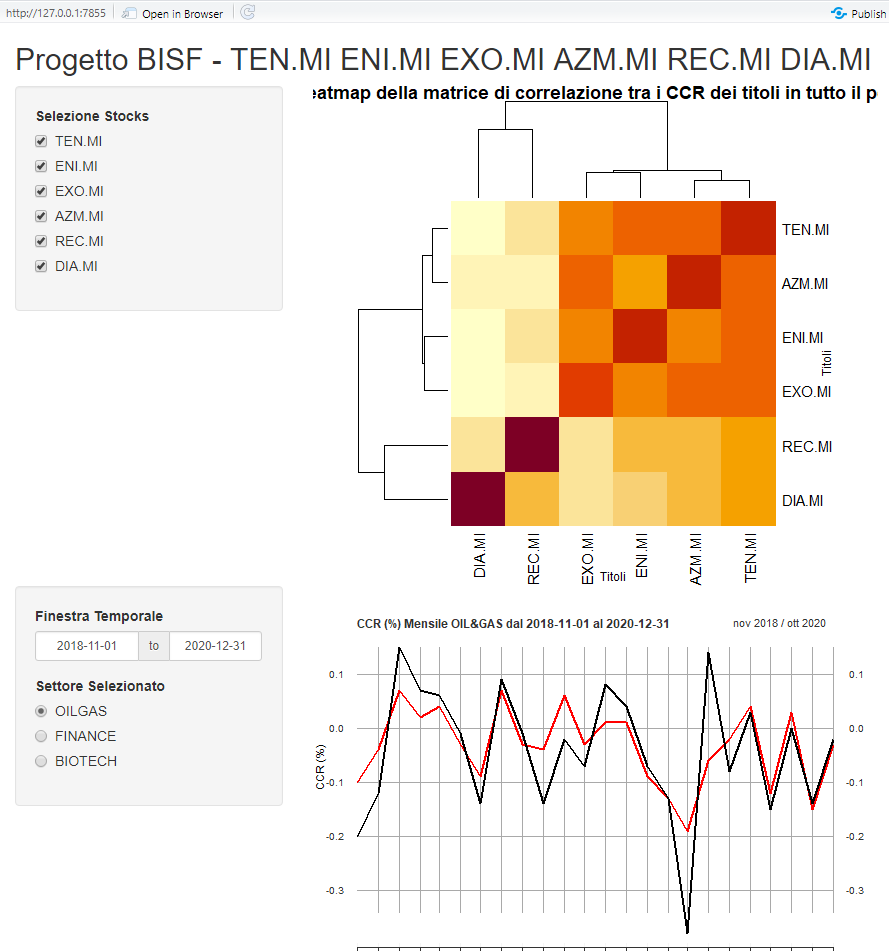
\includegraphics[width=0.9\textwidth]{immagini/WEBAPP.png}
    \caption{Screenshot Web App Shiny}
\end{figure}
\FloatBarrier
\end{document}